
\documentclass[12pt,a4paper]{article}
%-------------------------------------------
%---Packages--------------------------------
%-------------------------------------------
\usepackage[utf8]{inputenc}
%\usepackage[T1]{fontenc}
%\usepackage{txfonts}
\usepackage{amsmath}
\usepackage{amsthm}
\usepackage{amsfonts}
\usepackage{array}
\usepackage{amssymb}
\usepackage{blindtext}
\usepackage{caption}
\usepackage{color}
\usepackage{csquotes}	    %
\usepackage{enumitem}	    %pour mieux bosser avec les listes. ajoute option label
\usepackage[yyyymmdd]{datetime}        %pour définir date custom
\usepackage{etaremune}
\usepackage{environ}
\usepackage{fancybox}
\usepackage{fancyhdr} 	    % Custom headers and footers
\usepackage{fancyref}
%\usepackage{float}
\usepackage{floatrow}       %float and floatrow can't be together...
\usepackage{gensymb}
\usepackage{graphicx}
\usepackage[colorlinks=true, linkcolor=purple, citecolor=cyan]{hyperref}
\usepackage{footnotebackref}
\usepackage{lipsum}
\usepackage{mathtools}
\usepackage{multicol}	    %gérer plusieurs colonnes
\usepackage{setspace}
\usepackage{subcaption}
\usepackage{todonotes}	    %Bonne gestion des TODOs
%TODO commenté pour tester l'utilité... à voir% \usepackage[tc]{titlepic}      %Permet de mettre une image en page de garde
\usepackage{tikz}	    % Pour outil de dessin puissant
\usepackage{ulem}	    %underline sur plusieurs lignes (avec \uline{})
\usepackage{vmargin} 	    %gestion des marges, avec dans l'ordre : gauche, haut, droit, bas, en-tête, entre en-tête et texte, bas de page, hauteur entre bas de page et texte
\usepackage{wrapfig}
\usepackage{xcolor}
\usepackage{xparse}                    %Pour utiliser NewDocumentCommand et des arguments 'mmooo'
%\usepackage{fullpage} 	    %supprime toutes les marges allouées aux notes, aussi en haut et en bas

%\ExplSyntaxOn
\pagestyle{fancyplain}	    %Makes all pages in the document conform to the custom headers and footers

%-------------------------------------------
%---Document Commands-----------------------
%---------------------------{----------------
\NewDocumentCommand{\framecolorbox}{oommm}
 {% #1 = width (optional)
  % #2 = inner alignment (optional)
  % #3 = frame color
  % #4 = background color
  % #5 = text
  \IfValueTF{#1}%
   {\IfValueTF{#2}%
    {\fcolorbox{#3}{#4}{\makebox[#1][#2]{#5}}}%
    {\fcolorbox{#3}{#4}{\makebox[#1]{#5}}}%
   }%
   {\fcolorbox{#3}{#4}{#5}}%
 }%
%------------------------------------------------
%------------------ENGLISH----------------------
%----------------------------------------------

\NewDocumentCommand{\epflTitle}{mO{Olivier Cloux}O{\today}O{Notes de Cours en}D<>{../../Common}}%Arguments : Matière, Auteur, Date, Titre du doc
{
\begin{titlepage}
    \vspace*{\fill}
    \begin{center}
        \normalfont \normalsize
        \textsc{Ecole Polytechnique Fédérale de Lausanne} \\ [25pt] % Your university, school and/or department name(s)
        \textsc{#4} %Titre du doc
        \\ [0.4 pt]
        \horrule{0.5pt} \\[0.4cm] % Thin top horizontal rule
        \huge #1 \\ % Matière
        \horrule{2pt} \\[0.5cm] % Thick bottom horizontal rule
        
\includegraphics[width=8cm]{#5/EPFL_logo}
        ~\\[0.5 cm]
        \small\textsc{#2}\\[0.4cm]
        \small\textsc{#3}\\
        ~\\
        ~\\
        
\includegraphics[scale=0.5]{#5/creativeCommons}
    \end{center}
    \vspace*{\fill}
\end{titlepage}
}


%-------------------------------------------
%-------------MATH NEW COMMANDS-------------
%-------------------------------------------
\newcommand{\somme}[2]{\ensuremath{\sum\limits_{#2}^{#1}}}
\newcommand{\produit}[2]{\ensuremath{\prod\limits_{#2}^{#1}}}
\newcommand{\limite}{\lim\limits_}
\newcommand{\llimite}[3]{\limite{\substack{#1 \\ #2}}\left(#3\right)}	%limites à deux condiitons
\newcommand{\et}{\mbox{ et }}
\newcommand{\deriv}[1]{\ensuremath{\, \mathrm d #1}}	%sigle dx, dt,dy... des dérivées/intégrales
%\newcommand{\fx}{\ensuremath{f'(\textbf{x}_0 + h}}
\newcommand{\ninf}{\ensuremath{n \to \infty}}	       %pour les limites : n tend vers l'infini
\newcommand{\xinf}{\ensuremath{x \to \infty}}	       %pour les limites : x tend vers l'infini
\newcommand{\infint}{\ensuremath{\int_{-\infty}^{\infty}}}
\newcommand{\xo}{\ensuremath{x \to 0}}									%x to 0
\newcommand{\no}{\ensuremath{n \to 0}}									%n zéro
\newcommand{\xx}{\ensuremath{x \to x}}									%x to x
\newcommand{\Xo}{\ensuremath{x_0}}										%x zéro
\newcommand{\X}{\ensuremath{\mathbf{X}} }
\newcommand{\A}{\ensuremath{\mathbf{A}} }
\newcommand{\R}{\ensuremath{\mathbb{R}} }								%ensemble de R
\newcommand{\rn}{\ensuremath{\mathbb{R}^n} } 							%ensemble de R de taille n
\newcommand{\Rm}{\ensuremath{\mathbb{R}^m} }  							%ensemble de R de taille m
\newcommand{\C}{\ensuremath{\mathbb{C}} }
\newcommand{\N}{\ensuremath{\mathbb{N}} }
\newcommand{\Z}{\ensuremath{\mathbb{Z}} }
\newcommand{\Q}{\ensuremath{\mathbb{Q}} }
\newcommand{\rtor}{\ensuremath{\R \to \R} }
\newcommand{\pour}{\mbox{ pour }}
\newcommand{\coss}[1]{\ensuremath{\cos\(#1\)}}						%cosinus avec des parenthèses de bonne taille (genre frac)
\newcommand{\sinn}[1]{\ensuremath{\sin\(#1\)}}					%sinus avec des parentèses de bonne taille (genre frac)
\newcommand{\txtfrac}[2]{\ensuremath{\frac{\text{#1}}{\text{#2}}}}		%Fractions composées de texte
\newcommand{\evalfrac}[3]{\ensuremath{\left.\frac{#1}{#2}\right|_{#3}}}
\renewcommand{\(}{\left(}												%Parenthèse gauche de taille adaptive
\renewcommand{\)}{\right)}
\newcommand{\longeq}{=\joinrel=}												%Parenthèse droite de taille adaptive


%-------------------------------------------------------
%------------------MISC NEW COMMANDS--------------------
%-------------------------------------------------------
\newcommand{\degre}{\ensuremath{^\circ}}
%\newdateformat{\eudate}{\THEYEAR-\twodigit{\THEMONTH}-\twodigit{\THEDAY}}



%-------------------------------------------------------
%------------------TEXT NEW COMMANDS--------------------
%-------------------------------------------------------
\newcommand{\ts}{\textsuperscript}
\newcommand{\evid}[1]{\textbf{\uline{#1}}}        %mise en évidence (gras + souligné)



%\newcommand{\Exemple}{\underline{Exemple}}
\newcommand{\Theoreme}{\underline{Théorème}}
\newcommand{\Remarque}{\underline{Remarque}}
\newcommand{\Definition}{\underline{Définition} }
\newcommand{\skinf}{\sum^{\infty}_{k=0}}
\newcommand{\combi}[2]{\ensuremath{\begin{pmatrix} #1 \\ #2 \end{pmatrix}}}	%combinaison parmi 1 de 2
\newcommand{\intx}[3]{\ensuremath{\int_{#1}^{#2} #3 \deriv{x}}}				%intégrale dx
\newcommand{\intt}[3]{\ensuremath{\int_{#1}^{#2} #3 \deriv{t}}}				%intégrale dy
\newcommand{\misenforme}{\begin{center} Mis en forme jusqu'ici\\ \line(1,0){400}\\ normalement juste, mais à améliorer depuis ici\end{center}}	%raccourci pour mise en forme
\newcommand*\circled[1]{\tikz[baseline=(char.base)]{
            \node[shape=circle,draw,inner sep=1pt] (char) {#1};}}			%pour entourer un chiffre
\newcommand{\horrule}[1]{\rule{\linewidth}{#1}} 				% Create horizontal rule command with 1 argument of height

\theoremstyle{definition}
\newtheorem{exemp}{Exemple}
\newtheorem{examp}{Example}


%-------------------------------------------
%---Environments----------------------------
%-------------------------------------------
\NewEnviron{boite}[1][0.9]{%
	\begin{center}
		\framecolorbox{red}{white}{%
			\begin{minipage}{#1\textwidth}
 	 			\BODY
			\end{minipage}
		}
	\end{center}
}
\NewEnviron{blackbox}[1][0.9]{%
	\begin{center}
		\framecolorbox{black}{white}{%
			\begin{minipage}{#1\textwidth}
 	 			\BODY
			\end{minipage}
		}
	\end{center}
}
\NewEnviron{exemple}[1][0.8]{%
    \begin{center}
        \framecolorbox{white}{gray!20}{%
            \begin{minipage}{#1\textwidth}
                \begin{exemp}
                    \BODY
                \end{exemp}
            \end{minipage}
        }
    \end{center}
}
\NewEnviron{suiteExemple}[1][0.8]{%
    \begin{center}
        \framecolorbox{white}{gray!20}{%
            \begin{minipage}{#1\textwidth}
                \BODY
            \end{minipage}
        }
    \end{center}
}
\NewEnviron{colExemple}[1][0.8]{%
    \begin{center}
        \framecolorbox{white}{gray!20}{%
            \begin{minipage}{#1\columnwidth}
                \begin{exemp}
                    \BODY
                \end{exemp}
            \end{minipage}
        }
    \end{center}
}
\NewEnviron{example}[1][0.8]{%
    \begin{center}
        \framecolorbox{white}{gray!20}{%
            \begin{minipage}{#1\textwidth}
                \begin{examp}
                    \BODY
                \end{examp}
            \end{minipage}
	}
    \end{center}
}
\NewEnviron{systeq}[1][l]{
			\begin{center}
				$\left\{\begin{array}{#1}
					\BODY
				\end{array}\right.$
			\end{center}
 }





%-------------------------------------------
%---General settings-----------------------
%-------------------------------------------
\renewcommand{\headrulewidth}{1pt}										%ligne au haut de chaque page
\renewcommand{\footrulewidth}{1pt}										%ligne au pied de chaque page
\setstretch{1.6}
\author{Olivier Cloux}


\renewcommand{\contentsname}{Table of Contents}
\begin{document}
\setstretch{1}
\epflTitle{Computer Networks}[Olivier Cloux][Fall 2015][Lectures Notes in]
\newpage
\begin{multicols}{2}
	\tableofcontents
\end{multicols}
\setstretch{1.2}
\setcounter{section}{-1}
\begin{boite}
	\begin{center}
		\evid{Notations and Conventions}
	\end{center}
	\begin{itemize}
		\item 1 byte = 1 "octet" = 8 bits
		\item Mbps = Mega \uline{bits} per second
		\item MBps = Mega \uline{bytes} per second
	\end{itemize}
\end{boite}

\section{Introduction and disclaimer}
Thank you for downloading and reading this document. Before you start, there are a few things I want to warn you about. First of all, this is a purely home-made document. Not official, not emitted by any official entity (as EPFL) or teacher. This represents my very own summary of the lectures on Computer Network, taken in Fall 2015 at EPFL. Then, very important, I'm not responsible for any kind of problem you might encounter. Some subjects in the lectures might change in the following years, this document might contain a few mistakes or need precisions (nobody is perfect),... It is all possible. If you fail your year/subject/... it's because of you. If course change (and it will), I probably won't take time to modify it (unless I have personal interest in doing so, or to correct inaccuracies/mistakes). As I said, the only goal of this document is to help me to remember everything, do revisions before exam and, if possible, help a few fellow students out there. 

This document is brought to you freely. I don't take any remuneration on it. Sharing some/all of this document is allowed and encouraged, as long as you don't have any financial/... compensation for it or take credit for the creation of the document. I would enjoy if you informed me before sharing on your website/drive/... but it is not mandatory.

That being said, I deeply hope you enjoy the present document ; if you see any mistake, inaccuracies,... please feel free to contact me at \href{mailto:olivier.cloux@epfl.ch}{olivier.cloux@epfl.ch}. I will be glad to correct the document if necessary

\evid{Last compilation of the present document : \today}
\section{Computer Networks and the Internet}
A network is mainly composed of 3 parts : end-systems (computer, cars, smartphones,...), switches (to redirect the connections) and links, between switches, systems,... Links can be various, as it is just a data connection : WiFi, phone cable, TV cable,... We will talk about networks in general, so it is not Internet connection by definition. To evaluate networks, we will consider packets, going from an end-system to an other, through those links and switches.
\begin{figure}[!h]
	\centering
	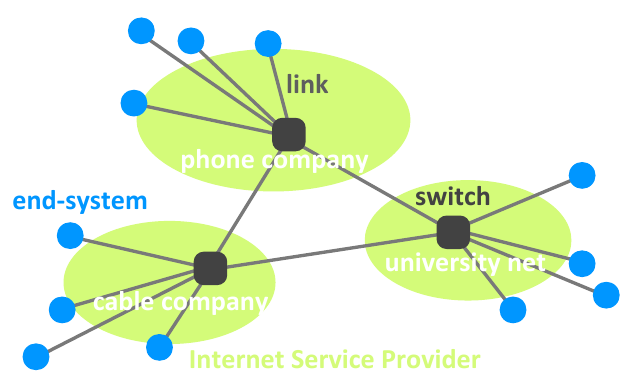
\includegraphics[scale=0.5]{images/general_system}
	\caption{A simplification of a network}
	\label{fig: general network}
\end{figure}
Most components (switches, cables but also servers,...) are mainly owned by \textbf{ISP} (internet service providers). ISPs can be phone companies, university networks, cable companies,...

\subsection{A few systems}
DSL (Digital Subscriber Line) is a type of connection. Links are made of twisted pair copper, with 3 separate channels : Downstream data (1$\sim$100 Mbps), upstream data (1$\sim$10 Mbps) and a 2-way phone channel.
\begin{figure}[!h]
	\centering
	\begin{subfigure}[b]{0.33\textwidth}
		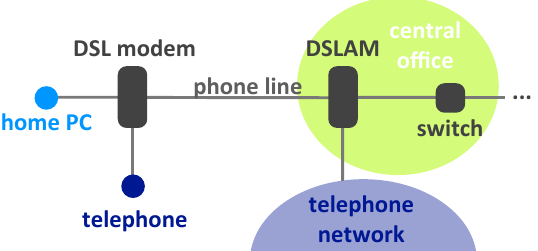
\includegraphics[scale=0.45]{images/dsl}
		\caption{A home network}		
		\label{fig: home DSL}
	\end{subfigure}
	~
	\begin{subfigure}[b]{0.33\textwidth}
		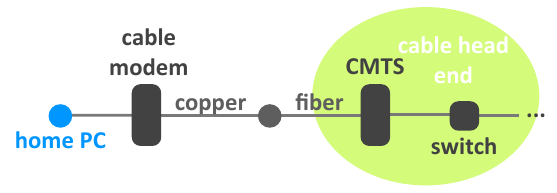
\includegraphics[scale=0.45]{images/cable}
		\caption{Cable network}		
		\label{fig: cable}
	\end{subfigure}
	~
	\begin{subfigure}[b]{0.33\textwidth}
		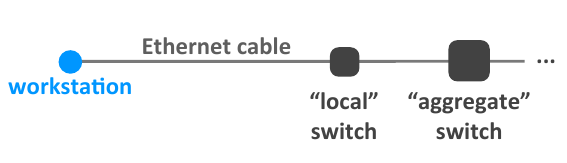
\includegraphics[scale=0.45]{images/uniNet}
		\caption{University network}		
		\label{fig: university network}
	\end{subfigure}
	\caption{Simple networks}
	\label{fig: simple networks}
\end{figure}
With cable however, we have a coaxial copper \& fibre, we really boost the upstream data channel, with now $\sim$10 Mbps. Ethernet is still the most efficient, with twisted pair copper, and tens of Gbps in each direction. We do not rely on a powerful sender (even if very efficient, we can't apply it to long cables, for ISPs)

\subsection{Switches}
A switch is composed, usually, of a buffer (small memory) to store data and a forwarding table to store meta-data\footnote{informations/data about data}(given an address, it knows approximately where to send the packet)

\subsubsection{Packet Switching}
Packets are processed in the switch (treated on demand), and sent to the right address, packet after packet. Provides an efficient resource use, but unpredictable performances. If the idea is right, we can't predict if many people want to connect at the same time, and thus flood the switch. In such a case, the buffer will fill, and when full, he will simply drop packets (definitely lost). For this system, we need \textbf{congestion control}.	

\subsubsection{Circuit Switching}
Connection switching through physical circuits. We send meta-data saying we want to connect to a certain point, and the resources are reserved in advance. Provides predictable performances, but a poor efficiency of resource use.\\
\evid{Frequency Division Multiplexing (FDM)} : Each user gets \textit{continuously a fraction} of bandwidth.\\
\evid{Time Division Multiplexing (TDM)} : Each user gets \textit{periodically the full} bandwidth
\begin{exemple}
	Suppose users share a 3 Mbps link. Each user requires 150 kbps when transmitting. What is the maximum of users, with a FDM and a TDM ?
	\begin{itemize}
		\item With a FDM : Each gets a fraction $\to \frac{3000\ kbps}{150\ kbps} = 20$ users 
		\item Everybody has the full bandwidth, periodically. Time is divided frames, each frame has U timeslots, each frame is T sec long. Thus, a user will send $(T\cdot 150)$ K-bits during his timeslots, and might send \textit{up to} $(3000 \frac{T}{U})$ kbits during that timselot. So, 
		\[T \cdot 150 \leq 3000 \frac{T}{U} \to U \leq 20\]
	\end{itemize}
	So any system will allow 20 users at most.
\end{exemple}

\subsection{Organization of a network}
\begin{figure}[!h]
	\centering
	\begin{subfigure}[b]{0.45\textwidth}
		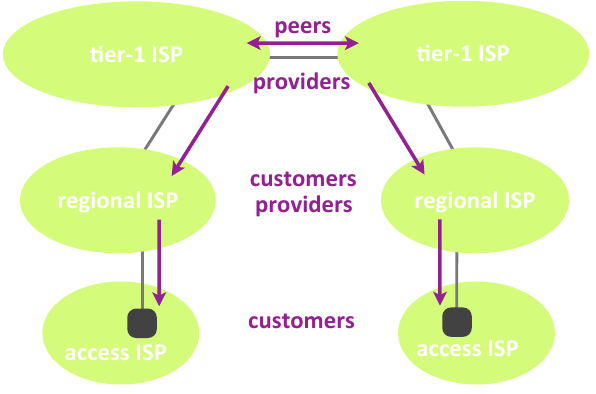
\includegraphics[scale=0.45]{images/ispsName}
		\caption{Naming of ISPs}		
		\label{fig: name of ISPs}
	\end{subfigure}		
	\quad
	\begin{subfigure}[b]{0.45\textwidth}
		 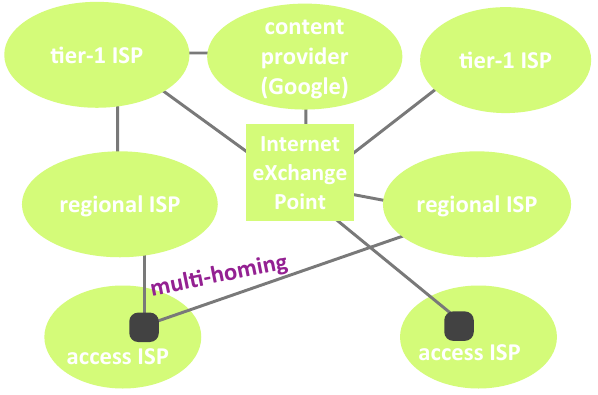
\includegraphics[scale=0.45]{images/isps}
		 \caption{ISPs} 
		 \label{fig: isps}
	\end{subfigure}
\end{figure}

\subsection{Layers}
\begin{figure}[!h]
	\centering
	\begin{subfigure}[b]{0.5\textwidth}
		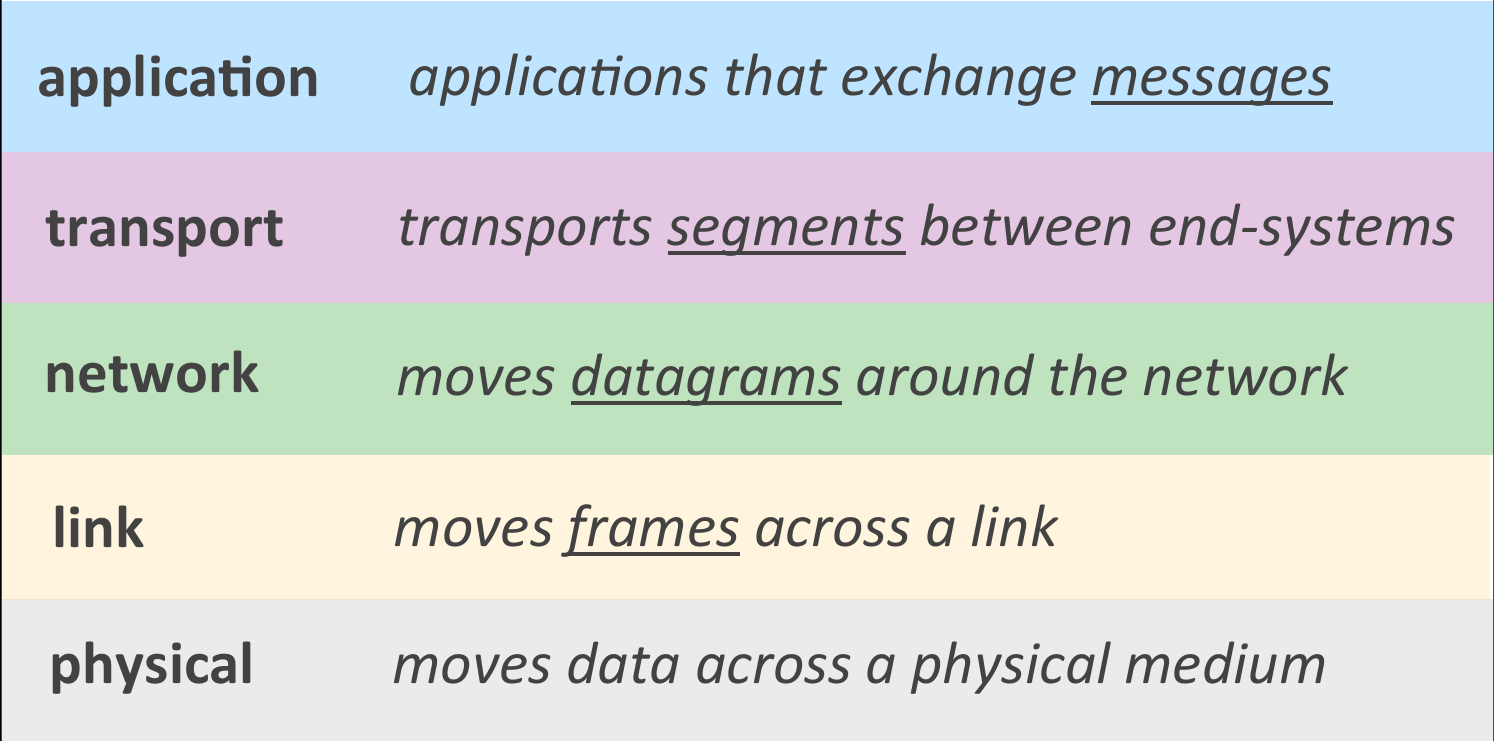
\includegraphics[scale=0.21]{images/layer_Name}
	\end{subfigure}
	\begin{subfigure}[b]{0.4\textwidth}
		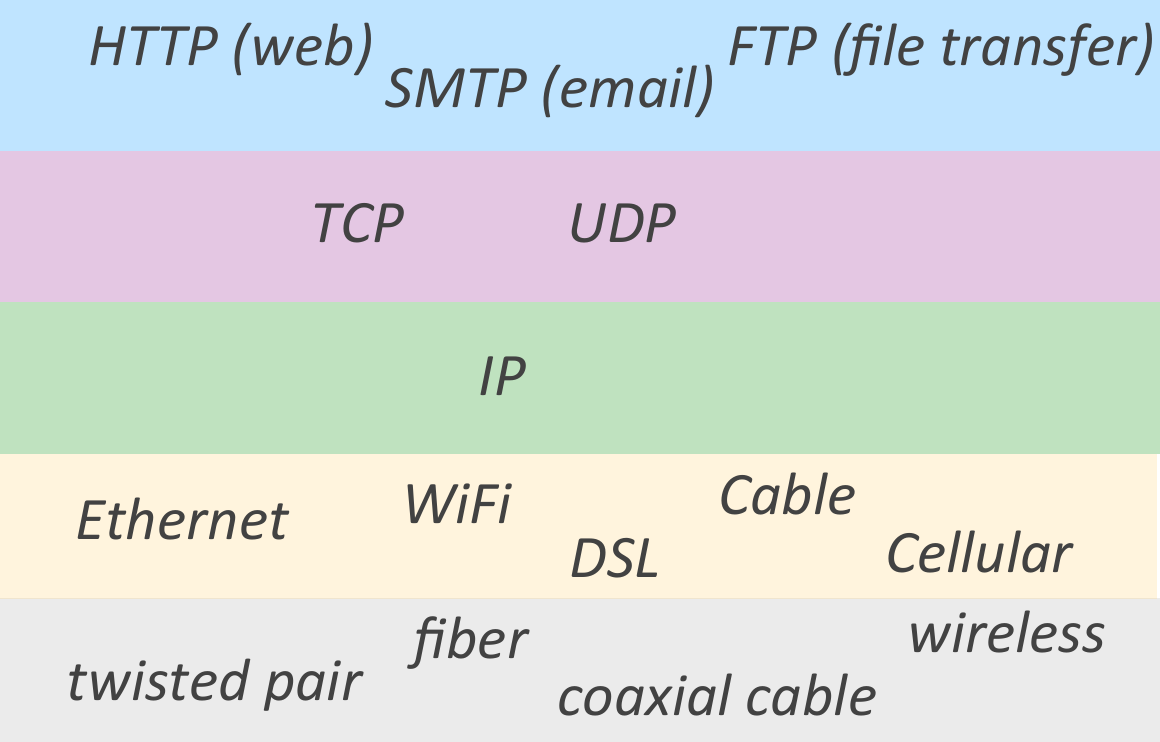
\includegraphics[scale=0.21]{images/layer_Protocol}
	\end{subfigure}
	\caption{The usual layers system used}
	\label{figs: layers}
\end{figure}
When sending a packet, each layer applies a header, with meta-data. Once the message arrived at the receiver's, the packet goes up 1 layer, gets its header removed, \uline{goes back to physical}, goes one higher, gets one more header removed, etc. until the messages arrives at the application layer, without any header.

\subsection{Delay}
\begin{enumerate}
	\item 	\textbf{Transmission delay} : how long does it take to push all the bits of a packet into a link ? 
			\begin{equation}
				\txtfrac{Packet Size}{Transmission rate of the link}
				\label{eq: transmission delay}
			\end{equation}						
	\item 	\textbf{Propagation delay} : how long does it take to move one bit from one end of a link to the other? 
			\begin{equation}			
				\txtfrac{Link Length}{Propagation speed of link}
				\label{eq: propagation delay}
			\end{equation}
	\item 	\textbf{Queuing delay} : how long does a packet have to sit in a buffer before it is processed ? 
	\item 	\textbf{Processing delay} : How long does to take to process a packet ?
\end{enumerate}
\evid{Note :} The product between the transmission rate of a link, and the propagation delay is the max amount of bits that can be in the link at a given time. 
\begin{exemple}
	Two hosts are separated by 20'000 Km and are connected with a link of $R = 2$ Mbps. The propagation delay over the link is $2.5 \cdot 10^8$ meters/sec. Thus, the product $R\cdot d_{prop} = 160'000$ bits, which means the link can't contain more than 160 Kbits at once. 
\end{exemple}

\subsubsection{Throughput}
At what rate is the destination receiving data from the source ? The average throughput is defined by :
\begin{equation}
	\txtfrac{Data size}{Transfer time}
\end{equation}

We can do an \uline{approximation}  of the transfer time, by dividing the size of the file by the smallest transmission rate. Of course, this is not accurate as we don't consider propagation delay, store-and-forward delay,... But we can say for sure that this smallest rate is the average throughput : if rates before and after this bottleneck are higher, everything will be limited by this part. That's why it is important to have constant performances.
\begin{exemple}
	Let's take 2 hosts A and B, connected by a switch, and 2 links of transmission rates R and R', with $R  < R'$. The first link automatically becomes a \textbf{bottleneck}. At which rate will the receiver receive the file ? At the smallest rate on the path, R. The transfer time will also be approximated with $\frac{F}{R}$
\end{exemple}

\subsection{Security}
\subsubsection[Eavesdropper]{Eavesdropper (sniffing)}
Trying to listen in on the communication to obtain copies of the data

\subsubsection[Impersonator]{Impersonator (spoofing)}
Pretending to be someone else (e.g. pretend to be a bank, to extract sensible informations from somebody)

\subsubsection[DoS]{Denial of Service (dos-ing)}
Flood a part (switch or server) to make one/both part crash, or just disconnect and disrupts the communication. Doesn't destroy anything permanently, just causes the connection (usually a server) to crash for a moment. Can be prevented, by blocking the IP address of the attacker. A \textit{distributed DoS} is much more dangerous : many infected end-systems participate in the flooding at the same time.

\subsubsection{Malware}
Contaminate a terminal, for various purpose, including :
\begin{itemize}
	\item 	Delete file on the terminal
	\item 	Copy and export personal data (keylogger,...)
	\item 	Send spam emails
	\item 	Launch or participate in a distributed DoS
\end{itemize}

\section{Application Layer}
When we want to design an application, we have to think about multiple things : the design of the architecture (which process does what ?), the design of the communication protocol (what sequences of messages can be exchanges ?) and the choice of the transport service (what delivery guarantee are needed ?)
\subsection{Architecture}
How will you share/send your data ? A dedicated server, running 24/7, treating every requests for a given data ? Or share your parts of your data with many peers, and then letting them share with each others ? We have to take in consideration what we want and need. A Peer-to-Peer for an online game server ? Worst idea ever. A client-server for sharing heavy files, such as films ? Better have really good servers. Let's analyse these two possible architectures.
\subsubsection{Client-Server}
Servers are taking requests from clients. One server is at a constant address, and clients type this address to reach the server. With many clients, you must have many servers too ; however, clients don't know that, they just connect to the data center. 

\subsubsection{Peer-to-Peer}
Both clients have a process that can make and answer requests. Each peer is the client AND the server. Each can request service from an other peer, or provide to an other. They run on end-structures (computer, tablet,...), no dedicated infrastructures. To design an application, we have to chose which architecture is better.

\subsubsection{How to choose ?}
\begin{figure}[h]
	\centering
	\begin{subfigure}[b]{0.45\textwidth}
		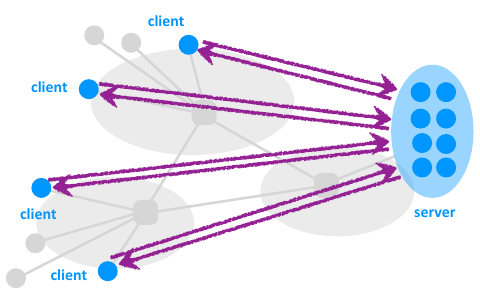
\includegraphics[scale=0.6]{images/clientServer}
		\caption{A Client-Server architecture}
		\label{fig: client server arch}	
	\end{subfigure}
	~
	\begin{subfigure}[b]{0.45\textwidth}
		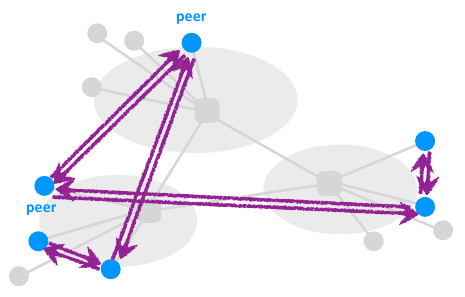
\includegraphics[scale=0.6]{images/p2p}
		\caption{A Peer-to-Peer architecture}
		\label{fig: p2p arch}
	\end{subfigure}
	\caption{The possible architectures}
	\label{figures: p2p and client-server architectures}
\end{figure}
Each architecture has advantages. For example, client-server will provide speed guaranteed and reliability, \uline{as long as the server is not flooded}. The most important here is the availability : you can be sure the server has what you want, but you rely on the availability of the server (up and running or not). With P2P, you \textit{may} have a faster download, if lot of people have what you want, and are ready to share ; but is nobody has it yet, you may rely on a handful of people, that might not be ready to share at a given moment, and thus your connection will be really small. Furthermore, with client-server, you can count and restrict what you send, which is harder (nearly impossible) with P2P, as you are not the only one sending. 


In summary : you have to consider the restraint you want to impose on the data, what max amount of connections you are expecting, at what frequencies you will change your data (a film is great in P2P as i will never change, but for an online game it is terrible) and the security of the data (again, a film is ok but a snapchat-like, going through 10 phones before yours, is terrible).

\subsection{Communication protocol}
\textit{What are the possible message exchanges between client \&  server or peers ?}.  qqThe chosen protocol is a part of the application you design : Protocol $\subset$ Application. Application = communication protocol + client \& server (or peer) processes + ...
\begin{exemple}~\\
	$\begin{array}{lcl}
	\text{Web } = & &  \text{ HTTP communication protocol} \\ 
	& + &\text{ web browser \& server processes} \\ & + &\text{ HTML language}
	\end{array}$
\end{exemple}

\subsection{Transport Service}
An application might have various expectations, regarding to the connection : You want your message to be extremely correct ? You want it to arrive really fast ? To be totally secured ? 
\begin{itemize}
	\item 	Reliable message delivery : The message is delivered to the destination process. If not, a failure signal is sent. It is for web pages, file transfer, email,... We say that those are \textbf{loss-sensitive applications}
	\item 	Guaranteed performance : We want a minimum throughput ; for example, using a video chat (skype,...) with someone, you don't want your application to be laggy, so you request a \textit{minimum throughput}. Your application is then \textbf{throughput-sensitive}. You might want also a \textit{maximum end-to-end packet delay} (again : sykpe,...). You don't want to talk, and your partner to respond to you 5 minutes later. Your application is then \textbf{delay-sensitive}.
	\item 	Guaranteed security : You might care about the security of your message. Can it be listened ? If yes, can it be understood (is is crypted) ? 3 point are to be looked at : the message is revealed only to the destination (\textbf{confidentiality}), the message is not changed along the way (\textbf{data integrity}) and the message indeed came from claimed source (\textbf{authenticity}).
\end{itemize}
For that, we use 2 internet transport services : \textbf{TCP}, that provides reliable message delivery and \textbf{UDP}, for which we don't have any expectation (but is usually much faster)

\subsubsection{TCP}
\begin{itemize}
	\item 	TCP code at the \textit{server machine} keeps a record with information about \textit{each active client process}.
	\item 	TCP code at the \textit{client machine} keeps a record with information about \textit{the server process}. 
\end{itemize}

"TCP is said to be \textbf{connection oriented}, because before one application process can begin to send data to another, the two processes must first \textbf{handshake} with each other (they send preliminary segments to each other to establish the parameters of the ensuing data transfer."\footnote{From the reference book, page 231} 

That's why we say that TCP is connection-oriented, or stateful, meaning it maintains state on communicating processes.

\evid{Non-Persistent TCP} : Typically only used by older web clients and servers. It adds overhead by connecting for each request. If the server has a limited number of parallel connections, it can be a better use of the resources. Used also for mobile-based application that contacts rarely the server.

\evid{Persistent TCP} : less delay experienced by the client (as he doesn't have to wait for the setup of each connection). Used by web browsers and chap-applications with "push-simulation" 

\evid{Multiple TCP connections} : asks for multiple connections to a server. The server can thus handle less clients simultaneously (as a server has a limited number of connections) but increase bandwidth instantaneously. Only most modern browsers use it, and download-helper.
\subsubsection{UDP}
UDP is really different. It only stores the address of the client/server, it doesn't keep any state about the packets, lost packets are not retransmitted. But why do that ? Well, if you want to sent an information ASAP, you typically don't want TCP. It will first perform a handshake, and then every packet will be verified, and sent again if necessary. That's why UDP is used in \uline{time-critical applications}, like voice transmission, or video chat. This service is said \textbf{connection-less}, or stateless.

\subsection{Examples}
\subsubsection{The Web} 
\uline{The architecture} is clearly client-server (with \nameref{subs: caching}) . A server has it's own informations, always evolving. When one does want to know about a website, the hosting server sends the related informations. At the server's, a process is always running, it is reachable at a fixed, known process address. It serves web pages, each with it's own URL (an address for internet resources).
	
\uline{The communication protocol} is \textbf{HTTP requests and responses}. Requests types are GET (request to download), POST (client provides information), PUT (client requests to upload a file) or DELETE (client requests to delete a file). The responses types are various : Ok, Not Found, Moved Permanently, Bad Request,... each with a code (Not found is 404, Ok is 200,...)

\begin{figure}[h]
	\centering
	\begin{subfigure}[b]{0.45\textwidth}
		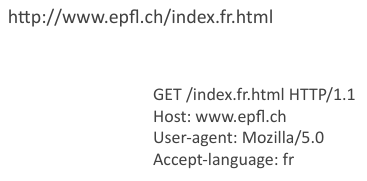
\includegraphics[scale=0.6]{images/requestHTTP}
		\caption{A typical GET request}
		\label{fig: get request}
	\end{subfigure}
	~
	\begin{subfigure}[b]{0.45\textwidth}
		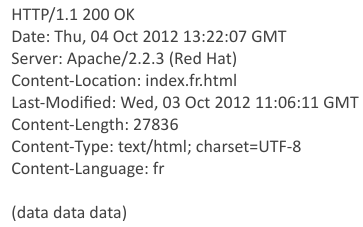
\includegraphics[scale=0.6]{images/responseHTTP}
		\caption{The corresponding response}
		\label{fig: http response}
	\end{subfigure}
	\caption{A GET request and it's response}
	\label{figures: get + response}
\end{figure}

\begin{exemple}
	A note about cookies : many websites use cookies. They are a little piece of information, stocked on your end-system. At first connection, a cookie is stocked in your browser. Then, every time you connect to this site, or make a request, the cookie will be sent with. It is usually used to "improve" your experience on a site. With that, one can know for example where you come from, your name, what type of products you like,... and then use these informations to give you more pertinent responses.
\end{exemple} 

Finally, the \uline{transport service} used is TCP (typically with persistent TCP connections).

\subsection{Caching} \label{subs: caching}
If a user wants to access a far server, connection will be slower (more distance, usually more switches,...). But once it is done, the information is most likely to be stored in a \textbf{proxy web server}, closer to the client. Thus, if he (or someone else) wants to access this same page shortly after, he just has to asks the proxy. It adds a new parameter to the GET request : if done to a proxy, we must also ask "if-modified-since:...". It the site hasn't been modified since, we download directly from the cache.

\begin{figure}[h]
	\centering
	\begin{subfigure}[b]{0.55\textwidth}
		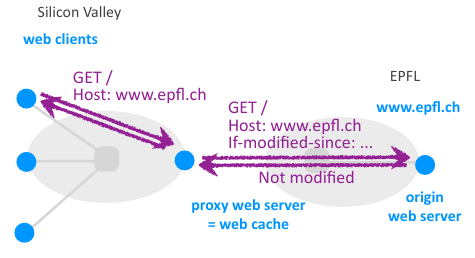
\includegraphics[scale=0.7]{images/proxy}
		\caption{A proxy}
		\label{fig: proxy scheme}
	\end{subfigure}
	~
	\begin{subfigure}[b]{0.4\textwidth}
		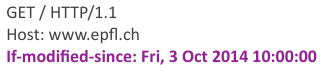
\includegraphics[scale=0.7]{images/getProxy}
		\caption{The associated GET request}
		\label{fig: proxy get}
	\end{subfigure}
	\caption{What a proxy looks like}
	\label{figs: proxy}
\end{figure}
\subsection{DNS}
When you want to reach a website, you usually asks with it's "human" name (e.g. www.epfl.ch). No one wants to remember an IP address. So before to ask to www.epfl.ch, you first want to know it's IP address. So you ask a \textbf{DNS server} the corresponding address. It will give you an answer, and you can then ask to the correct address.

But you can't have only one worldwide DNS server that remember every address, not even one per country, remembering all servers in a specific country. Too easy to attack, too propitious for a failure, too hard for maintenance. That's why DNS servers are organised in a hierarchy (see Figure \ref{fig: DNS hierarchy}) : \textbf{Roots} servers talk to \textbf{TLD} servers, who talk to \textbf{Authoritative} servers.
\begin{figure}[h]
	\centering
	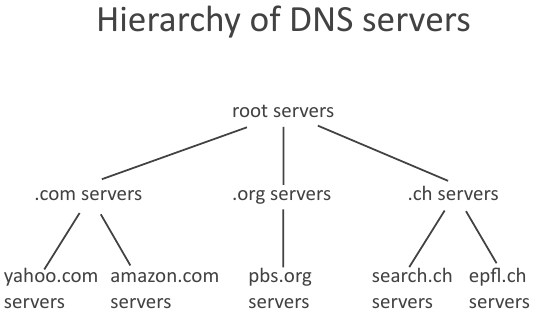
\includegraphics[scale=0.5]{images/dns_Hierarchy}
	\caption{The DNS hierarchy}
	\label{fig: DNS hierarchy}
\end{figure}

So basically we have 2 way to go through this hierarchy : either \textit{recursively} (each DNS server asks next one ; once one has the information, it gives to the one who asked, until client) or \textit{iteratively} (if a DNS server doesn't have the answer, it will give a negative answer to the client, with the name of another server who might have the answer). See Figure \ref{figs: DNS iterative + recursive}

\begin{figure}[h]
	\centering
	\begin{subfigure}[b]{0.45\textwidth}
		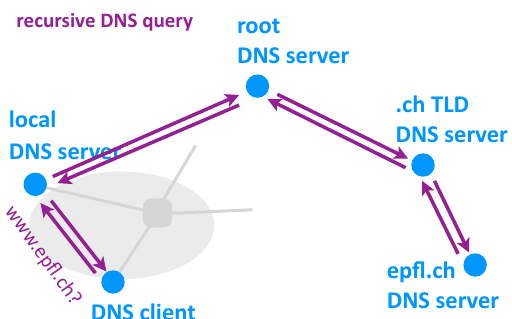
\includegraphics[scale=0.5]{images/recursive_DNS}
		\caption{A recursive query}
		\label{fig: recursive DNS}
	\end{subfigure}
	~
	\begin{subfigure}[b]{0.45\textwidth}
		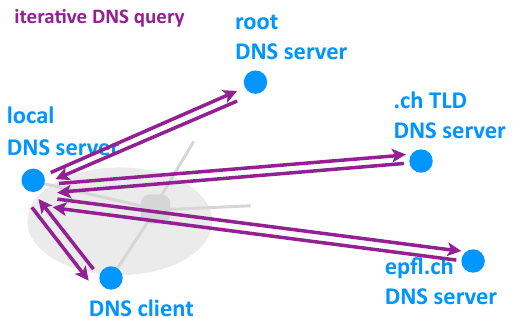
\includegraphics[scale=0.5]{images/iterative_DNS}
		\caption{An iterative query}
		\label{fig: iterative DNS}
	\end{subfigure}
	\caption{The difference between recursive and iterative queries}
	\label{figs: DNS iterative + recursive}
\end{figure}

We can note that DNS servers use \nameref{subs: caching} at all levels (once a server is asked for a domain, may it be root or local, it will stock the answer until it becomes too old). As an application, DNS are client-server, for DNS client - local DNS server as well as for local DNS server - rest of the hierarchy. This application of course uses UDP.

\subsubsection{Attack}
To attack the DNS system, you might :
\begin{itemize}
	\item 	Flood a client with "answers" to a question, waiting him to ask. He will then take your fake message for an official answer. You can then redirect him to your own server, and use impersonation to make him believe you are someone else. Not efficient, you must know what query will be made,
	\item 	Use a good old (D)DoS on any DNS server. They will then be unable to communicate. 
	\item 	Finally, you can flood a server with false queries, which will "poison" the cache. Not really useful, you will only make the servers have to ask until the authoritative server, increasing the delay experienced by the client.
\end{itemize}

\subsection{BitTorrent}~
\begin{figure}[!h]
	 \centering
	 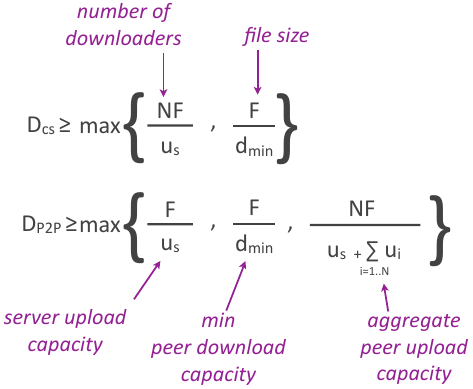
\includegraphics[scale=0.5]{images/download}
	 \caption{Download between Client-Server (CS) and Peer-to-Peer (P2P)}
	 \label{fig: download p2p}
\end{figure}

The main problem here, is to connect a peer who wants some data, to a peer that has these data. For that we will use 
\begin{itemize}
	\item 	\textbf{trackers} (=servers), who are nodes that keep track of which peers have the given content.
	\item 	Set of peers, through \textbf{DHT} : distributed structure that keeps track of which peers have what content 
\end{itemize}
\subsubsection{DHT}
For each content (say, film title), translated to a unique identifier, to an end-system (say, Alice, Bob,...), translated to a unique identifier like an IP address ; then, these correspondences are stocked in various servers, who communicate with each other. Each server knows a few other servers 

\section{Transport Layer}
Don't mess with network layer : 
\begin{itemize}
	\item 	Transport layer is a logical communication between \uline{processes}
	\item 	Network layer is a logical communication between \uline{hosts}
\end{itemize}
\evid{The analogy of the household :} 12 kids sending letters to 12 kids \\
Processes = kid, app messages = letters in envelopes, hosts = houses, transport protocol = Ann and Bill, network-layer protocol = postal service
\subsection{(De)Multiplexing}
Multiplexing and demultiplexing is quite simple to understand. Multiplexing (at sender) is ability to send information to multiple peers,
\begin{figure}[h]
	\centering
	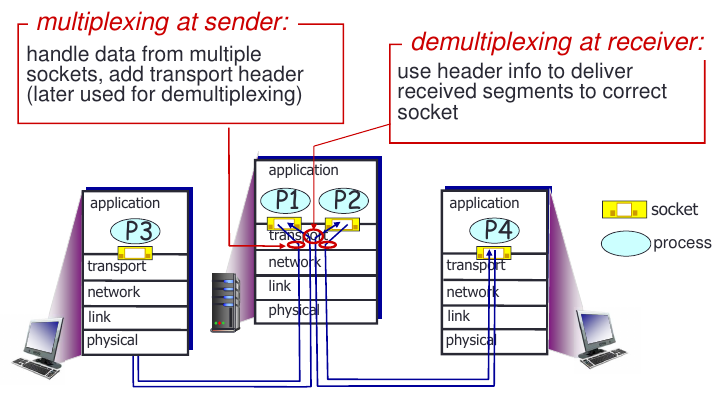
\includegraphics[scale=0.6]{images/multi_demulti}
	\caption{Multiplexing and Demultiplexing, at server}
	\label{fig: multi/demulti}
\end{figure}
%\ref{
while Demultiplexing (at receiver) is the ability to receive from multiple peers. When sending information to a receiver, the sender (server) will add a particular header that will be given back in the answer ; this is essential to associate a peer with the right process.

\subsubsection{Demultiplexing}
\evid{Connectionless} is when you use UDP packets. For that, every UDP packet will receive destination IP address + destination port number ONLY. Once Alice receives the packet, she simply keep sending packets to the same address as she did before. All packets (from everyone) will be directed to the same socket (and process). 

\begin{figure}[h]
	\centering
	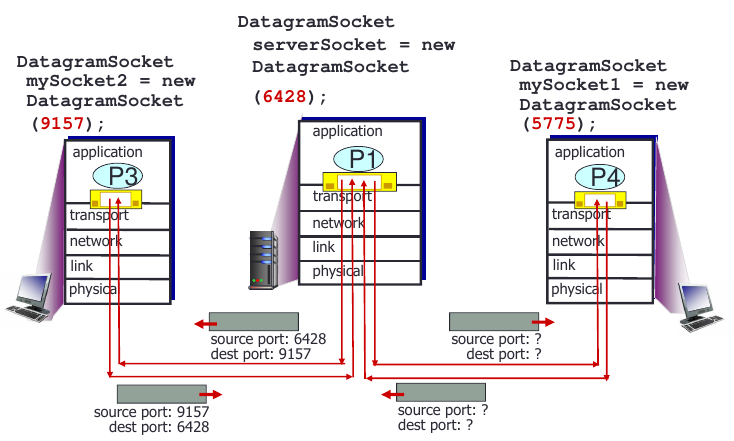
\includegraphics[scale=0.5]{images/exemple_header_demultiplexing}
	\caption{What a connectionless demultiplexing will look like}
	\label{fig: header_demu}
\end{figure}

\evid{Connection-oriented} is when you use TCP packets. Here, when a server responds to Alice, he has to specify the usual destination port and IP, and add a return address (an source IP address and port number). The server has a "welcome socket", used by default. Once he responds, he specifies a new port number (and maybe new IP address). This port is now dedicated to Alice. At the end of the connection, the port is freed and can be allocated to someone else. Let's note that for a persistent HTTP, we associate different socket for each connecting client, while for non-persistent HTTP, we have a different socket for each request.

\begin{figure}[!h]
	\centering
	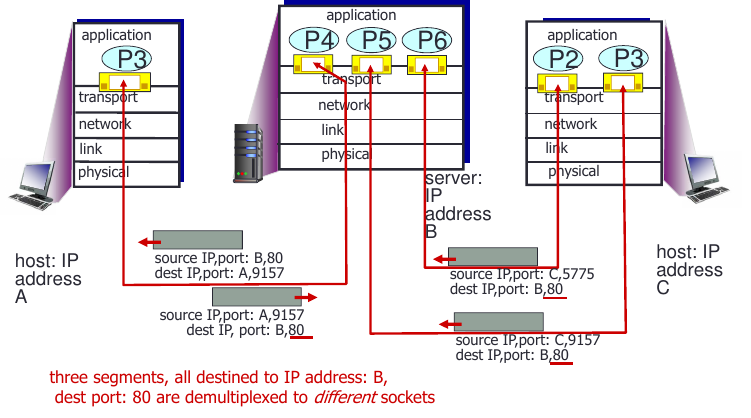
\includegraphics[scale=0.6]{images/tcp_demu}
	\caption{What a connection-oriented demultiplexing will look like}
	\label{fig: tcp_demu}
\end{figure}

\subsection{Socket}
Generally, a socket is the \textbf{interface} between application and transport layer. It can be UDP (unreliable, datagram) or TCP (reliable, byte-stream oriented). UDP is more "send this ASAP", while TCP is more secure, for reliable result.

\subsubsection{UDP}
\begin{figure}[!h]
	\centering
	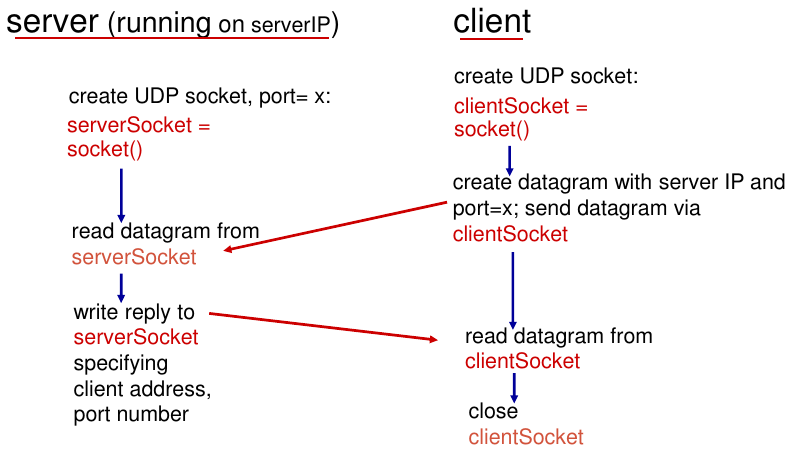
\includegraphics[scale=0.5]{images/udp_sequence}
	\caption{The client and server action sequences for a UDP interaction}
	\label{fig: udp_sequence}
\end{figure}
As said earlier, no persistent connection is kept between client and server. There's no handshake before sending data, and sender only attaches IP address and port number of the destination to each packet. Be careful, as some data may be lost, or received too late (out of order), because there's no verification of data integrity. In a network as big as Internet, loss or big delay are frequent, usually because of switches being full (a congestion). We can see what a sequence of actions in UDP will look like at Figure \ref{fig: udp_sequence}.
\newpage

\subsubsection{TCP}
Client process must first contact the server ; for that, the client creates a socket (used for later connection) specifying IP address and port number of server process (of the welcoming socket), and then send a request. This will establish a connection to server TCP (called the \textbf{handshake}). Server \uline{must} be already running ; it will receive the request, create a socket (the communication socket) that will be used to communicate with that particular client. Client IP and port numbers are used to distinguish clients. See the corresponding sequence of actions at Figure \ref{fig: tcp_sequence}.
\begin{figure}[!h]
	\centering
	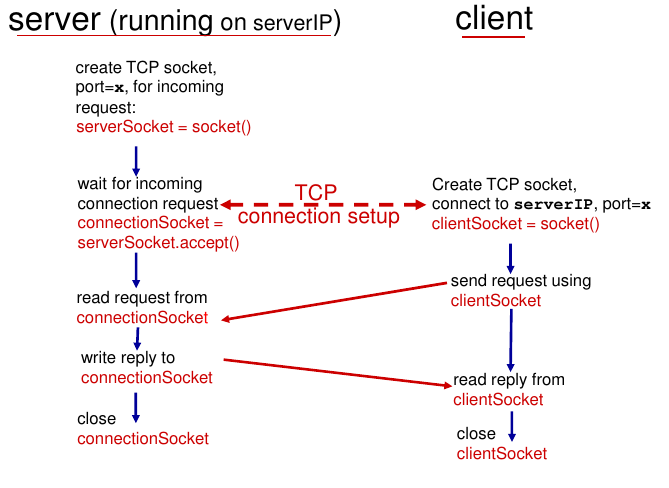
\includegraphics[scale=0.5]{images/tcp_sequence}
	\caption{The client and server action sequences for a TCP interaction}
	\label{fig: tcp_sequence}
\end{figure}

\section{Network Layer}
The transport layer is in between the application and network layer. Transport is a \textit{reliable data transmission} (rdt), while network uses \textit{unreliable data transmission} (udt). Basically :
\begin{enumerate}
	\item  	The application uses a rdt\_send() on a message to pass it to the transport layer.
	\item 	This layer adds a Header, and uses udt\_send to pass it to the network layer
	\item 	Message is transmitted through network, to arrive at the receiver's machine.
	\item 	Transport layer uses rdt\_rcv() (the transport is reliable)
	\item 	Finally, deliver\_data() to transmit to the application layer.
\end{enumerate} 
\evid{The question of reliability :} The message might arrive but with errors, or missing bites. We use \textbf{a checksum} (like the sum of bites of the segment) to check the correctness of a message. If sum and the checksum are not equal, the message is incorrect. Checksum might even be used to correct errors.\\
\evid{(N)ACK} = (negative) acknowledgement. If message is correct $\to$ ACK, if message is detected incorrect $\to$ NACK

\begin{figure}[!h]
	\centering
	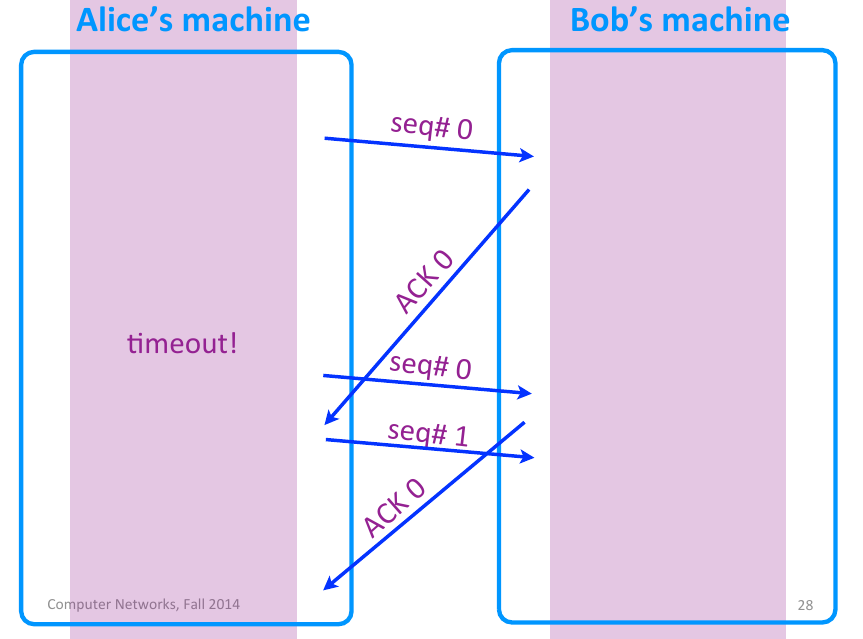
\includegraphics[scale=0.3]{images/suspicious_ack}
	\caption{ACK0 arrives immediately after sending seq\#0... strange !}
	\label{fig: ack timeout}
\end{figure}

\evid{Timing} : if a confirmation arrives late (or suspiciously early, see Figure \ref{fig: ack timeout}), the answer is not expected any more, or it might cause troubles. If after sending a packet, no (N)ACK came, the packet is sent again. The timeout is used to \textit{overcome data loss}\\
\evid{Summary} 3 elements are important :
\begin{itemize}
	\item 	Checksum : to detect (and correct) data corruption at receiver
	\item 	ACKs + retransmissions : to overcome data corruption
	\item 	Timeout + ACKs + retransmission : to overcome data loss.
\end{itemize} 

\subsection{Stop-And-Wait protocols}
\begin{figure}[!h]
	\centering
	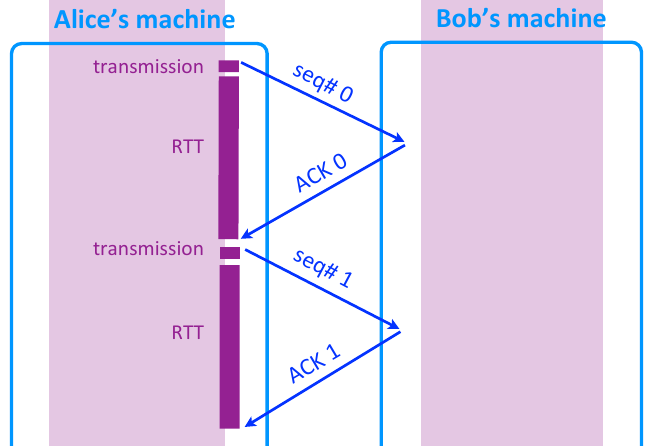
\includegraphics[scale=0.4]{images/stopAndWait}
	\caption{A basic \textit{Stop-And-Wait} protocol}
	\label{fig: stop and wait}
\end{figure}
Most basic protocol. A segment is sent, a (N)ACK is sent back. In case of a NACK or a timeout, the segment is sent again. There are multiple problems here : first, the sender does nothing while waiting for an (N)ACK, thus the system becomes really, really slow. That's why we define them as \textit{poor sender utilization}. Timeout and NACKs are used to overcome data loss \& corruption.


\subsection{Pipelining protocols}
The \textit{Stop-And-Wait} protocols, as seen above, are not efficient enough. Better protocols can be created, using \textbf{pipelining}. Pipelining (from the visualisation of filling a pipeline) has consequences for RDT protocols :
\begin{itemize}
	\item 	The range of sequence numbers must be increased, since each in-transit packet (not counting retransmissions) must have a unique sequence number and there may be multiple, in-transit, unacknowledged packets.
	\item 	The sender and receiver sides of the protocols may have to buffer more than one packet. Minimally, the sender will have to buffer packets that have been transmitted but not yet acknowledged. Buffering of correctly received packets may also be needed at the receiver, as discussed below.
	\item 	The range of sequence numbers needed and the buffering requirements will depend on the manner in which a data transfer protocol responds to lost, corrupted, and overly delayed packets.
\end{itemize}
Pipelining protocols are defined by a \textit{good sender utilization} : while we wait for a (N)ACK, we keep sending segments. We send up to N un-ACKed segments, with N = sliding window size.
Here are the 2 main pipelining protocols.
\subsubsection{Go-Back-N}
Here, the idea is that the receiver won't accept a packet (nor stock it) if the precedent hasn't arrived yet. Thus, the ACKs are \textit{cumulative}, (if the sender receives ACK\#7, it means the receiver did correctly receive packets up to 7 (included !).
\begin{figure}[!h]
	\centering
	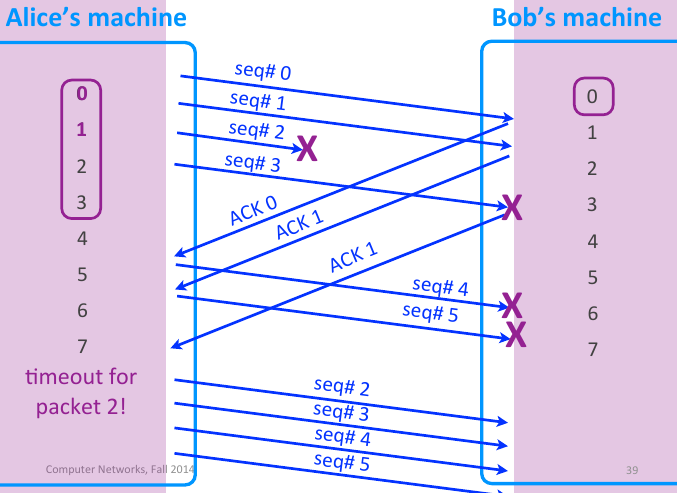
\includegraphics[scale=0.4]{images/goBackN}
	\caption{A \textit{Go-Back-N} protocol}
	\label{fig: Go-Back-N}
\end{figure}
In case of a NACK or a timeout, the sender will send every segments that haven't been ACKed yet.
As the receiver won't accept an "out-of-order" packet, when such a packet arrives, receiver drops it and send again the last ACK  he could.
\subsubsection{Selective Repeat}
Here, the receiver will accept any segment. If a precedent hasn't arrived yet, the receiver will stock (in a buffer) incoming segments until the missing one arrives. To make that possible, the ACKs must be \textit{selective} (an ACK\#7 only means that segment 7 has arrived)
\begin{figure}[!h]
	\centering
	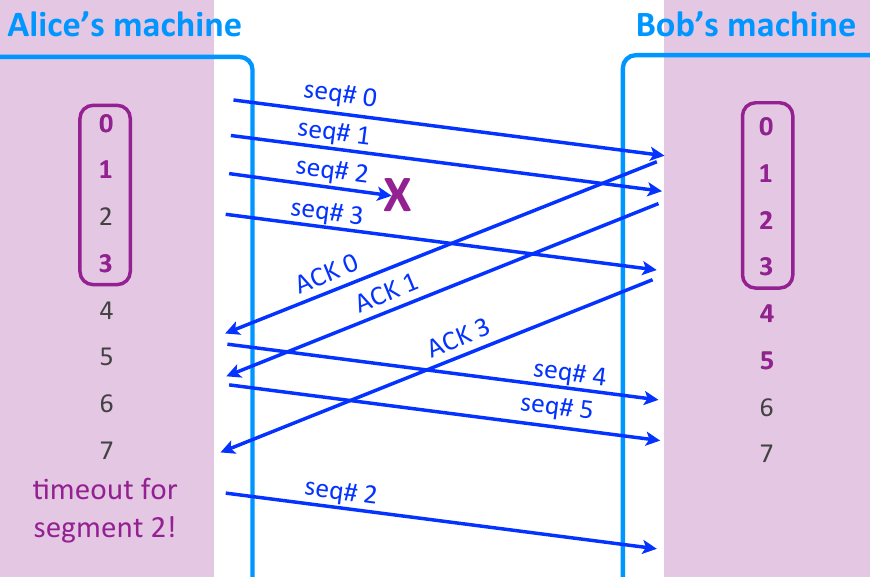
\includegraphics[scale=0.4]{images/selective}
	\caption{A \textit{Selective Repeat} protocol}
	\label{fig: selective repeat}
\end{figure}


%%%%%%%%%%%%%%%LECTURE 7%%%%%%%%%%%%%%%%%%%%%%%%%%
\section{More on TCP}
\subsection{TCP connection}
A TCP connection is made of 3 things :
\begin{itemize}
	\item 	A socket (to pass information between app-layer and TCP)
	\item 	2 buffers : send and receive buffer, to store sent/received data (it is called a bidirectional
	\item 	Variables (we'll talk about it later)
\end{itemize}
TCP is a 3-way handshake : the client initiates the process with a \textit{connection request}, server responds with a \textit{request acknowledgement} and finally client answers with an \textit{ack. of request ack.}.

\subsection{Reliability}
When starting a TCP connection, you must be sure every bits arrived, in the good order. For that purpose, TCP joins 2 additional values : \textbf{Sequence number} (SEQ), provided by data sender, represents the number of first byte of data (if no data, pretend there is some) and \textbf{Acknowledgement number} (ACK), provided by data receiver, represents the number of oldest byte expected by receiver (cumulative\footnote{As mentioned earlier, an ACK is cumulative if receiving ACK x means all bytes until x (included) were correctly received.}). Those two are always present, even when they are not needed (for example, you want to acknowledge a packet without sending anything ; simply pretend you will send some, and ACK ; later you send same SEQ/ACK tuple but with data).

\begin{figure}[h]
	\centering
	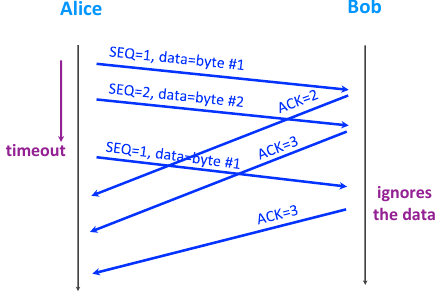
\includegraphics[scale=0.5]{images/timeout}
	\caption{How timeout works}
	\label{fig: timeout}
\end{figure}

Travelling through large networks, it is probable that a packet gets dropped (lost) or corrupted. That's why sender sets a \textbf{timeout} system : when sending a packet, it expects an ACK in some time. If it doesn't get an ACK in time, it will try to send again. If the original packet is corrupted/dropped, no ACK will be sent, sender timeouts and send again. If ACK gets lost, sender timeouts and send again ; as it already received the packet once, receiver will simply ignore the packet and retransmits most emitted ACK. You can see an example of timeout in Figure \ref{fig: timeout}.

In order to be efficient, timeout should occur a little bit after one RTT. It will allow enough time for segment to reach receiver and ACK to reach sender. But how can one predict the RTT ? For that, you take a sampleRTT (tome for a single RTT), and then compute the following :
\begin{itemize}
	\item 	EstimatedRTT = 0.875 EstimatedRTT + 0.125 SampleRTT
	\item 	DevRTT = function(RTT variance)
	\item 	Timeout = EstimatedRTT + 4 DevRTT
\end{itemize}
This computes an empirical, conservative prediction of RTT.

\subsubsection{Retransmission}
Let's be efficient : you send many packets at once (the \textbf{sending window}) and wait for ACKs. But your second packet got lost. You will then receive an ACK for the first one (named ACK2), then 3 times ACK2 again (as he will still wait for second packet). At this point, you use \textbf{fast retransmit} : sender receives 3 duplicate ACKs (meaning a segment was lost or delayed), it will then retransmits segment with oldest un-ACKed sequence number (instead of all segments). Sender will practice retransmission in because of 2 possible events : first, it timeouts ; it means a segment or an ACK was corrupted, lost or delayed. Second, it receives 3 duplicate ACKs, meaning one segment (you know which one, last un-ACked) was corrupted, lost or delayed.

\subsubsection[GBN/SR]{Go-Back-N ? Selective-Repeat ?}
With all these elements, you can decide if TCP is Go-Back-N or Selective repeat : actually it is a hybrid. As in GBN, ACKs are cumulative and it does not ACK individual out-of-order segments, but as SR, sender retransmits only one segment.

\subsection{Flow Control}
New problem : we always considered the receiver had an infinite receiving buffer, on infinite speed. But that's not real. If you receive too fast, the buffer will overflow and you simply lose packets. Not good. We now add a new data to the header : the size of receiver window. At beginning of connection, receiver sends, along to the packets, the size of receiver window. From now on, sender can send as many packets as he wants, as long as the sum does not exceed this window... until new information. Because with the ACK, of all those packets, there is the updated size of receiver window. When size is 0, there is an exchange of empty SEQ and ACK, until receiver window gets greater than 0. You can see a good example in Figure \ref{figs: window size}

\begin{figure}
	\centering
	\begin{subfigure}[b]{0.45\textwidth}
		\centering
		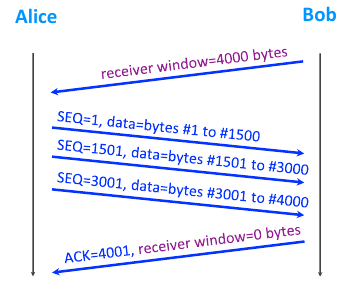
\includegraphics[scale=0.8]{images/window_ok}
		\caption{Sending up to the window size}
		\label{subfig : receiver window ok}
	\end{subfigure}
	~
	\begin{subfigure}[b]{0.45\textwidth}
		\centering
		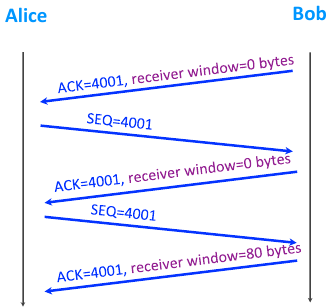
\includegraphics[scale=0.8]{images/window_full}
		\caption{Waiting for window to enlarge}
		\label{subfig : receiver window full}
	\end{subfigure}
	\caption{Example of window size use}
	\label{figs: window size}
\end{figure}

The goal of this procedure is to slow down the sender, so the receiver can follow.

\subsection{Security}
Let's look at some more aspects of security. One man try \textbf{TCP hijacking}. In other words, it would mean answering with an evil answer before the real ACK, causing for example the redirecting to a false html page. The best defence against this is to randomize sequence numbers. With that, Jack the hijacker can't just answer with a most probable SEQ and ACK, as it would make no sense for the sender. You can answer only if you can read it.

One can also use \textbf{SYN flooding}. Sending loads of SYN segments to a server, requesting each time a SYNACK segment (but without answering those SYNACKs). The server's socket would quickly overflow, avoiding anyone to complete a real TCP request. Best defence : use non-forgeable tickets and getting rid of the SYN buffer. You need a buffer to conserve the state of the client (time of request, IP,...) but you can get rid of that if you send back a ticket that can't be modified containing this state. Get rid of buffer, get rid of this attack.
\subsection{Congestion Control}
We know the problem of queuing delay. Before a bottleneck, in the switch, the buffer might be filled until the point packets get dropped. Other problem : even if the packet is not dropped, it might wait for a very long time in the buffer, causing Alice to timeout... even if he packet hasn't been dropped ; she will send again, causing the switch to do useless retransmissions. If n people use a link with a bottleneck R, Alice will have a throughput of R/n. But part of that rate is spent on retransmission, causing her \textit{effective throughput} to be inferior to R/n.

As seen, congestion has really bad effects. Long queuing delays and resource waste (sender has to retransmit, router transmit duplicate packets, routers transmit packets that will be dropped by receiver,..). A way to avoid this is to create a \textbf{congestion window}, representing the number of un-ACKed  bytes that the sender my transmit. 

The best way to determine the maximum sender window size, is to compute the \textbf{bandwidth-delay product} (rate R $\times$ delay before first ACK). This is the max amount of traffic the sender can transmit until he gets the first ACK.

We understood, the traffic on the network is really variable. We can't just determine a window size, and stick to it for the rest of our life. That's why we use \textbf{self clocking}. As long as we receive ACKs, there is no congestion and thus can increase the window. But when ACKs stop arriving, it means there is congestion and we must decrease the window. When we expect no congestion, it's OK to increase the window size \textit{exponentially} (by 1 MSS for every ACKed MSS). But when we expect congestion, we grow \textit{linearly} (by one MSS every RTT)

\subsubsection{TCP Reno}
This is the commonly used TCP algorithm. We will only discuss about some generalities. First, we start growing the window exponentially (this is called the \textbf{slow start)}. At some point, there will be a congestion, sender times out, resets the window to MSS and set a \textbf{congestion threshold} to  \txtfrac{last window size}{2}. But now, we can estimate a point to which we will switch from exponential to linear growth (alias \textbf{congestion avoidance)}. This point is either when window reaches congestion threshold, or when sender receives 3 duplicate ACKs\footnote{This last condition is specific to Reno ; an other protocol, Tahoe resets window to 1 after timeout when Reno resets to congestion threshold}

\subsection{Bonus}
That's a personal part, not included in the lectures. We will discuss an exercise in the 2013's final exam, in order to understand the chapter.
Here is the question : 
\paragraph{Consider the graph shown in Figure \ref{fig: 2013}, which shows the window size of a TCP sender as a function of time. a. Identify what happens to the congestion window at the following times : t=0.5, 3, 3.5 8 secs}
\begin{figure}[h]
	\centering
	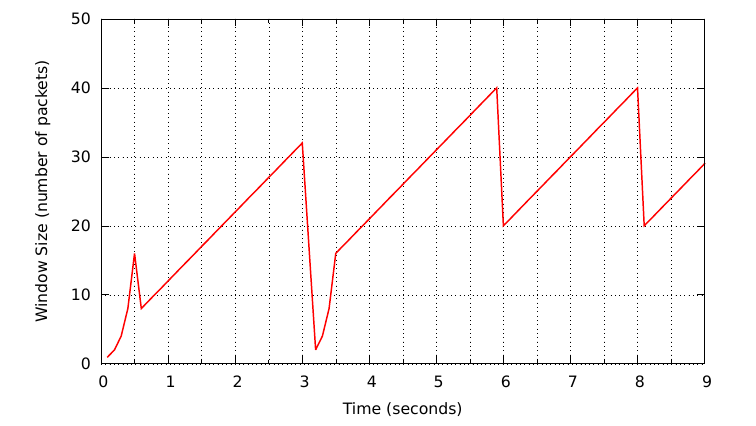
\includegraphics[scale=0.5]{images/2013}
	\caption{Congestion window size graph}
	\label{fig: 2013}
\end{figure}

Resolution :At t=0.5 secs, we have 3 duplicate ACKs. That's why the window size is set to half the size. The precedent state was "slow start" (exponential form), and we know that after 3 duplicate ACKs we are in state "Fast Recovery", so that's the state we are in. At t=3sec, we have a packet timeout, causing the congestion window to decrease to 1 TODO
\misenforme
%%%%%%%%%%%%%%%LECTURE 8%%%%%%%%%%%%%%%%%%%%%%%%%%
\section{Back on Network Layer}
\subsection{Network-layer functions}
Packets have to go from one end to an other. A big problem is : how do intermediate routers know where to send it ? They can't possibly know every end-point and routers in the world
\begin{itemize}
	\item Locally, we can set \textbf{Forwarding} : a \textit{local} router process that determines \uline{output link} for each packet ("with destination address x, forward to output link y").The router looks at the header and looks for a match in it's forwarding table.
	\item In a bigger view, we set \textbf{Routing} ; this is a \textit{network-wide} process that determines the \uline{end-to-end path} for each packet (content of forwarding table). This process can be distributed (each router runs it at the same time) or centralized (one server rules the world).
\end{itemize}

The \textbf{connection setup} is a \textit{path-wide} process that sets up connection state in routers.

\subsection{Network-layer services}
Out of the possible guarantees we might want to assure, we will look at the \textbf{guaranteed minimum throughput}. In order to do so, we introduce the concept of \textbf{virtual circuit}
\subsubsection{Virtual Circuit}
This is a way to make easy some connection, a but like connection switching. You send your packet, with some unique ID and informations (like destination, speed needed), and the first switch will remember that and forward that info further. Later, when you want to repeat this setup, you simply send the ID, and connection will instantly be made. There are 2 ways to implement VC : with 3 or 4 numbers. You need, at each router, input link, output link, and incoming VC\#. With 3 numbers, we assign a \textit{globally unique ID} that is no 2 VC will have the same ID, so the router will know where to forward. The more realistic way is to use 4 numbers : an incoming and an outgoing VC\#. Routers assign a \textit{locally unique ID}, meaning the ID changes at every hops. Thus, routers only have to treat VC like a forwarding table, acting on VC\# and links, instead of just IP and links.

Note that this method is not used with the Internet, as it doesn't scale very well.
\subsection{IP forwarding ++}
\hypertarget{IP mask}
An IP address is a 32 bits long binary number, so going from 0 to $2^{32}-1$. It is separated in 4 block, each 8-bits long. (so each block has values from 0 to $2^{8}-1 = 255$. In order to use a range of IP address, we created IP prefix prefix format, with the form (for example) :
\[223.1.1.0/24\]
This will regroup all IP addresses whose 24 first bits match \[223.1.1 \sim 11011111.00000001.00000001\] The 8 remaining bits can be anything, the beginning still match. This "24" is called a \textbf{mask} and can be anything as $0 \leq \text{mask} \leq 32$. Note that there are many correct ways to write the same ting. All following are equivalent :
\begin{align*}
	223.1.1.0/24\\
	223.1.1.74/24\\
	223.1.1.113/24
	223.1.1.*\\
	11011111.00000001.00000001.*\\2
	11011111.00000001.00000001/24
\end{align*}
Note that the mask can be different from 24 and doesn't have to be a multiple of 8 (it can be 12 if you want). For example, setting $223.1.1.0/12$ will give you all addresses from $223.0.0.0 = \textcolor{red}{11011111.0000}0000.00000000.00000000$ to $223.15.255.255 = \textcolor{red}{11011111.0000}1111.11111111.11111111$. Anything as long as the 12 first bytes don't change.

\subsubsection{But why ?}
It is really useful for a router/switch to know where to forward packets. The idea is to set rules, like "all IP in this range must go to that link". This is the fastest way to know where to forward a packet.

Such tables can have "duplicates" addresses ; consider the following :
\begin{wraptable}{l}{9.5cm}
\centering
\begin{tabular}{|l l l |c|}
\hline
\multicolumn{3}{|c|}{dest. address range} & output link\\
\hline
0-2 & 0000-0010 & 00** & 1\\
3 & 0011 & 0011 & 2\\
4,6,7 & 0100, 0110, 0111 & 01** & 3\\
5 & 0101 & 0101 & 4\\
8-15 & 1000-1111 & 1*** & 5\\
\hline
\end{tabular}
\caption{An example of a datagram network table}
\label{tab: datagram network}
\end{wraptable}
 all computers in an enterprise are in a subnet, and the router switch connected to this enterprise knows `` all packets corresponding to subnet 00** must be forwarded to link 4''. But the president (0011) wants a direct link to the switch. Even though he is in the subnet, he as a different link. An additional rules is entered : address 0011 must go to link 5. The \ref{tab: datagram network} corresponds to such an example.
 
So now, how do we handle a packet addressed to Mr. President ? It corresponds to mask 00** but also to the precise address 0011\ldots In such a case, we apply the \textbf{most restrictive mask}, i.e. 0011. We might not encounter masks as 00** and 0*** in a single table, but in such a case, the rule of the most restrictive applies .
\subsection{The inside of an IP router}
Not seen in the slides ?


%%%%%%%%%%%%%%%LECTURE 9%%%%%%%%%%%%%%%%%%%%%%%%%%
\subsection*{Routing}

\subsection{Least-cost path routing}
\begin{figure}[h]
	\centering
	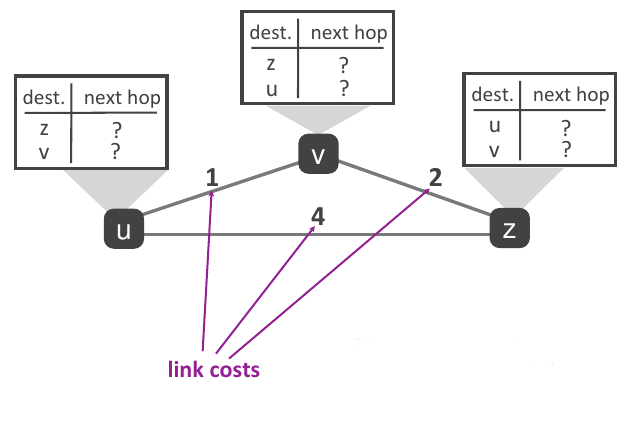
\includegraphics[scale=0.5]{images/router_graph}
	\caption{Representation of a small router graph}
	\label{fig: router graph}
\end{figure}
Now imagine a router graph (as in Figure \ref{fig: router graph}) : a few/lot of routers, some have links and each link has a cost\footnote{could represent propagation delay load}
This is a complex problem. Given a router graph and link cost, your goal is to find the least-cost path from each source router to each destination router. For that, you consider starting from a point (say, end system 10), and connect to closest router (say u). But this router now has to know where to send this bloody packet, and ASAP. He has to know what is the next \textit{hop} (next router), if possible do least cost possible. In order to succeed, you have 2 approaches : link-state routing or distance-vector routing.

\subsubsection{Link-state}
It uses Dijkstra's algorithm : the source router considers every other router. You first consider "how can i go to my neighbours" (in 1 hop), and remember the cost. Then go to smallest cost neighbour, and try again neighbours. If you can go to a router in a smaller cost than before, update former cost and "next hop". You can see an example of such an algorithm on Figure \ref{fig: example link state routing}. 
\begin{figure}[h]
	\centering
	\begin{subfigure}[t]{0.3\textwidth}
		\centering
		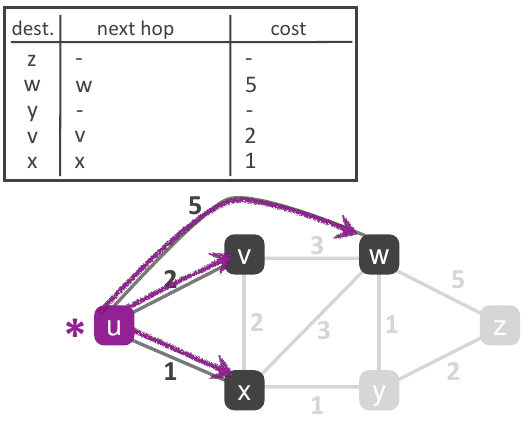
\includegraphics[scale=0.4]{images/dijkstra1}
		\caption{Step 1}
		\label{subf: step1}
	\end{subfigure}
	~
	\begin{subfigure}[t]{0.3\textwidth}
		\centering
		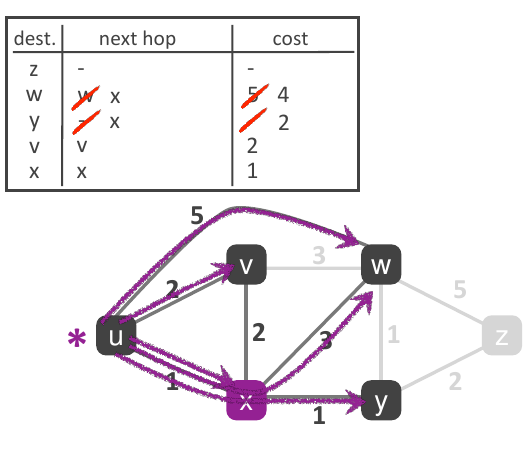
\includegraphics[scale=0.4]{images/dijkstra2}
		\caption{Step 2}
		\label{subf: step2}
	\end{subfigure}
	~
	\begin{subfigure}[t]{0.3\textwidth}
		\centering
		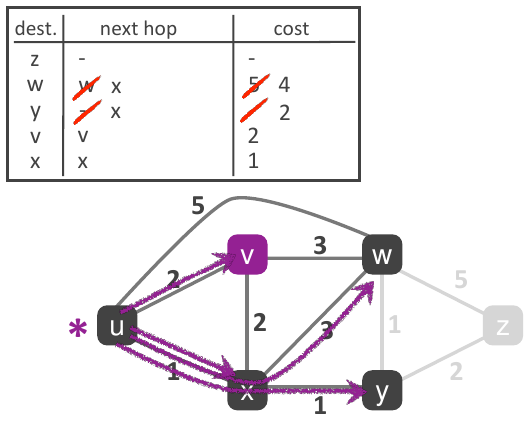
\includegraphics[scale=0.4]{images/dijkstra3}
		\caption{Step 3}
		\label{subf: step3}
	\end{subfigure}
	~\\
	\begin{subfigure}[b]{0.3\textwidth}
		\centering
		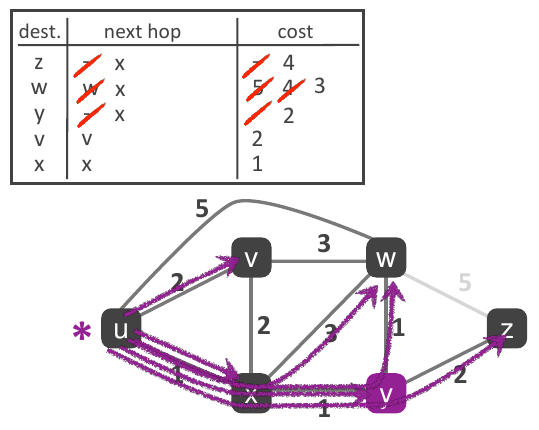
\includegraphics[scale=0.4]{images/dijkstra4}
		\caption{Step 4}
		\label{subf: step4}
	\end{subfigure}
	~
	\begin{subfigure}[b]{0.3\textwidth}
		\centering
		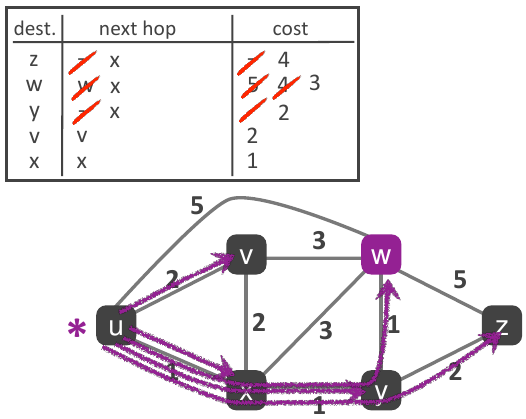
\includegraphics[scale=0.4]{images/dijkstra5}
		\caption{Step 5}
		\label{subf: step5}
	\end{subfigure}
	~
	\begin{subfigure}[b]{0.3\textwidth}
		\centering
		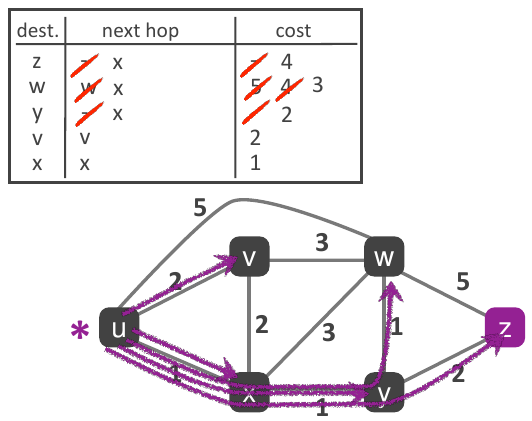
\includegraphics[scale=0.4]{images/dijkstra6}
		\caption{Step 6}
		\label{subf: step6}
	\end{subfigure}
	\caption{Link-state routing with Dijkstra's algorithm}
	\label{fig: example link state routing}
\end{figure}

On step 1, you fill the table with your neighbours, and respective costs. Then, continue on step 2 with cheapest neighbour (x), and explore close routers. Can you reach a node you already reached in a cheaper way ? Yes, w can now be reached in 4 instead of 5, and y can be reached. Restart from u : except already considered nodes (x), what is the closest neighbour ? v. Is there any improvement possible ? No. Do the same with next cheapest v's neighbours (steps 4,5,6), continuously update table. Tadaa, your table tells you the next hop for fastest way to all routers.

This is a \textit{centralized} algorithm (not distributed). You have 2 option : either your router runs it (computes least-cost path to every other routers) or or a separate machine runs the algorithm. It computes the least cost path between all routers.

\subsubsection{Distance-vector}
Here the idea is slightly different. You Keep a square matrix, with cost between 2 points. A router knows the cost to go to its direct neighbours. It first fills the (local) table with these informations. Then, it will ask its neighbours informations about their table. Doing that a few times will fill your table. But is is least-cost ? Most likely not. You might know that the path from z to x costs 7, and, somewhere in the table, you know that z-y is 1, and y-x is 2. Least-cost is then 3, going through y. That's the algorithm : try to improve by using intermediate nodes. Stop when no more improvement is possible. This is \textbf{Bellman-Ford algorithm}. Mathematically, this is expressed with the following :
\begin{equation}
	d_x(z) = \text{min}_n \{\text{cost}(x,n) + d_n(z)\} \quad \text{for all nodes }n
	\label{eq: Bellman-Ford}
\end{equation}
This algorithm is \textbf{distributed}, as all routers run it together (each runs an instance, and they exchange and react to each other's messages).

Now, this has a serious problem. If a link goes down (yeah, it can happen), you will probably get a routing loop ; consider following scenario : z routes through y, and y through x, y loses connectivity to x, so y decides to route through z. y will ask z "what is your cost to go to x ?" and z will give last known cost, the one going through y. Y will then take this cost. Seeing it changed, z will change too, then y, then z,\ldots this is a \textbf{count-to-infinity scenario}.

The solution : when you are done (when the path between x and z pass through y), you decide that "unused" links have an infinite cost. That way, when y-x goes down, y asks z best way to go to x, it will have choice between routing through y (from known informations, y said its route to x is infinite), or directly to z (obviously better). This will quickly re-converge, and avoids count-to-infinity scenario ; that is called \textbf{poisoned reverse}.


\subsection{Routing the Internet}
Those 2 methods are great, with advantages and problems, but have 2 problems : \uline{Scale} : having a table containing all routers of the network, which might be real big (consider every router of the Internet !) and \uline{Administrative autonomy} : an ISP may not want to do least-cost routing, and may want to hide its link costs from the world (along with other political difficulties). 

That's why we define \textbf{AS (Autonomous Systems)}, that are an ensemble of switches, routers, end-points that are all run by 1 ISP. Each AS runs its own routing algorithm \footnote{Intra-AS Routing} and can determine a path between every pair of routers inside the same AS. When a peer wants to send a packet to some IP address, it first checks if the IP is in the AS ---usually, AS are determined by an \hyperlink{IP mask}{IP mask}---; if it is, according to the path determined by the routing algorithm, if not send to an other (the right one !) AS.

There exists also an Inter-AS routing algorithm, that is run by all Internet routers, used to determine the path from each router to each IP prefix advertised by a foreign AS. This solution scales (each router does not have to know the position of every single router), and respects the administrative autonomy (ISPs use own routing algorithm, and don't have to reveal internal composition of AS).

\subsubsection{Internet Routing Protocols}
The two most famous Intra-AS routing protocols are RIP (Routing Information Protocol) and OSPF (Open Shortest Path First). The Inter-AS routing protocol is BGP


%%%%%%%%%%%%%%%LECTURE 10%%%%%%%%%%%%%%%%%%%%%%%%%%
\section{Security}
When sending a message, we might want to be assured one or some of these 3 points : \textbf{Confidentiality} : only the sender and receiver can read the message. \textbf{Authenticity} : the receiver is assured of the identity of the sender. \textbf{Integrity} : the message has not be changed along the way.
\subsection{Building Blocks}
The important point in confidentiality is \textbf{encryption/decryption}. We start with a plaintext, pass it through an encryption algorithm to get a cyphertext. Ideally, this cyphertext shoud not reveal anything about the plaintext. We then transmit it to the receiver, who uses a decryption algorithm to obtain the original plaintext.
\paragraph{Note : this part is real close to Sciences de l'Information. Good idea to go check my document about it}~
\\

The natural way to encrypt some text is to use a \textbf{symmetric key encryption}. We scramble the text in a certain way using a private key, and it then is easy to rearrange it using the same key. The problem happens when sharing. The challenge stand in making sure the key is transferred securely. 

Considering this sharing problem, we use \textbf{asymmetric encryption}. Here, the sender asks the receiver for a \textit{public key}, that anyone can read. It is impossible to decrypt the text using this key. The secured is then sent, and receiver uses a \textit{private key} to decrypt the text. It is more secured when using sharing, but is more resources-consuming !

In order to transfer messages faster, we can make messages shorter, using  hash function. With that, we map larger input to smaller hash. It should not reveal any information on input, and it should be hard to identify 2 inputs that lead to the same hash. It is different from encryption, in the sense it goal is not to be unreadable.

\subsection[Security Properties]{Providing security properties}
We said we first wanted to provide \textbf{confidentiality} : we can avoid \textit{Eve the eavesdropper} with asymmetric encryption. Even if she can intercept the message, she can't read it. We have a problem when \textit{Manuel the Man-in-the-Middle} intercepts the message. He can emit a new public key and transmit it to sender. Sender will use this key, and Manuel can intercept the message, decode it, modify it as it pleases him, encrypt it again using original key, and send it. No one will see shit.

Second problem, is providing \textbf{authenticity}. Asking your bank for infos, how can you be sure it is the bank ? And how can they be sure you are Alice ? Giving IP address with the message is not secured (you can fake it). Instead, Alice (you) send a public key, a message saying she is Alice and a cyphertext. Using the public key on the cypher will translate into "I am Alice"

\subsection{Securing Internet protocols}
TODO : Securint Email

\evid{Securing TCP :} Server sends its public certificate, and includes its public key. Client creates and sends a shared master key (with server's public key)


\section{Link Layer}
In a transport analogy (with tourists and shit), link represents the transport segment, and the transport mode is the link layer protocol. 

\subsection{Link-layer services}
This layer provides a \textbf{error detection}: detects errors caused by signal attenuation or some "noise", and drop frames with such errors ; it also provides \textbf{reliable data delivery}. It detects but also corrects/retransmits frames with error ; used for links with high-error rate (wireless). We also have \textbf{link access} (how to share the same link with other nodes) and \textbf{flow control} (pacing between adjacent sending and receiving nodes.
\subsubsection{Error detection/correction}
In order to detect errors (with very few chances to miss), we add some redundancy : EDC bits, i.e. bits that could represent sum of bits, or something else. With that, receiver computes same calculus as in the beginning and compares with given EDC. Difference means something went wrong. It's not 100\% reliable, but good enough. The larger the EDC field, the better the detection. 

A good way to use these EDC bits is to compute parity of a sequence. It can be done in one dimension (Figure \ref{subf : parity_1d}) or two dimensions (Figure \ref{subf : parity_2d})
\begin{figure}[h]
	\centering
	\begin{subfigure}[b]{0.45\textwidth}
		\centering
		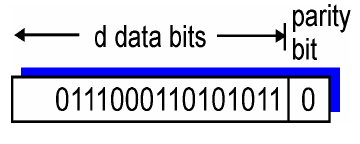
\includegraphics[scale=0.5]{images/parity_1d}
		\caption{1D}
		\label{subf : parity_1d}
	\end{subfigure}~
	\begin{subfigure}[b]{0.45\textwidth}
		\centering
		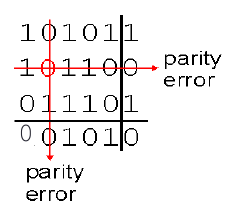
\includegraphics[scale=0.5]{images/parity_2d}
		\caption{2D}
		\label{subf : parity_2d}
	\end{subfigure}
	\caption{One and two dimensional bit parity}
	\label{figs: bit parity}
\end{figure}

But the most efficient is CRC, widely used in practice (Ethernet, WiFi)

\subsubsection{MAC}
Not the same as before. Means Media Access Control.

TODO

\subsubsection{CSMA}
Multiple nodes may use a link at the same time. So first you sense the channel. If idle, transmits, if busy, defer transmission.
TODO

\subsubsection{Turns}
A way to avoid multiple people on a link at once, we have 2 solutions : \textbf{polling} : a "master" invites "slaves" to transmit. Computer waits until the master invites him to transfer. But this represents a single point of failure. We can also use \textbf{token passing} : a control token is passed from one node to an other sequentially

\subsection{Link-layer forwarding ++}
\subsection{Transporting informations}
In order to send to an address, you use the MAC addresses. Those are used to move frames between link-layer nodes, and there exists exactly one MAC address per NIC. Their format is 48 bits address\footnote{Example : 71-65-F7-2B-08-53}, flat. The \textbf{broadcast address} is expressed as \[\text{ff:ff:ff:ff:ff:ff}\] 

When you want to send a packet to someone, you send to the MAC address. Every system has an \textbf{ARP table}, associating MAC addresses and IP addresses. And when you don't know the MAC of an IP, you make an \textbf{ARP request} : ask everyone in the subnet for a given IP. When you get the answer, you stock it in your table.
\subsubsection{Ethernet}
This represents the dominant and first widely used  wired connection LAN technology, 
TODO


\subsubsection{Switch}
It forwards frames within LAN, by determining output port based on \uline{destination MAC address}. It is similar to router forwarding process. It is also \textbf{self-learning} : it forwards table populated \uline{automatically}, there's no need for manual configuration or routing protocol. A table is usually empty at first, and each time a frame (from a specific MAC address) goes through the switch, it records the incoming link and MAC address, with a TTL. A \textbf{switch table} may look like this :
\[\begin{tabular}{|c|c|c|}
	\text{MAC address} & \text{Interface} & \text{TTL}\\
	\hline
	AD-17-E4-3D-11-87 & 1 & 60\\
	FF-31-2F-57-44-7B & 3 & 60\\
	\vdots & \vdots & \vdots
\end{tabular}\]
An important thing to know about switches and routers : they don't perform ARP queries. When they get a packet to forward, they either know the MAC address already, from previous transfers or simply "flood" the network. Only the sender perform ARP queries.
\begin{exemple}
	How does self-learning work ? given a network, all points connected to a single switch. It initially has an empty forwarding table. But after a while, A decides to send a packet to A'. For that, all packets have, in the header, the MAC address of destination and source. Not knowing where A' is, the router \textbf{floods} the network : everybody gets a copy of the packet, waiting for an answer. But with that, the switch received a packet, knowing the corresponding link and source address (header). So it can fill the table with one entry : packets for A go to this link. After a while, all points are in the table.
\end{exemple}


\section{Presentations last lecture}
\subsection{Dan Tomozei, Software engineer, Cisco}
PHD : Peer to peer systems (congestion control for p2p live streaming). PostDoc with \#JYLB ! Smart grids/integration of renewable energy in the power grid. 

Cisco made it possible to connect everyone, pushing for protocols like TCP/IP. Dan mostly does Software development at EPFL/Rolle.

Converged access : make the client believe he is in the same L2 network. How ? All clients traffic is encapsulated in a tunnel at the AP. Other endpoint is at the switch, "Rpoute" tunneled\ldots.

IOS : Cisco OS. Single core hardware (IOS was traditionally a single huge executable, suitable for routers, legacy codebase,..). On new hardware, you can use multicore : IOS is being split in processes running in a custom Linux. This is really hard (Huge codebase). building from scratch can take hours. 

Some features : AVC : Application Visibility and control : Deep packet inspection to determine which client applications use bandwidth (can be used to prioritize Sykpe over Youtube for example). Hyperlocation : Ability to physically locate wireless clients (in a mall, campus\ldots), by triangulation. 

\subsection{Electri-fi}
Demand for home connectivity is exploding. Call for additional technologies to boost up wifi. 	


\appendix
\section{Glossary}
\begin{multicols}{2}
\begin{enumerate}
	\item 	ACK : (usually positive) Acknowledgement
	\item 	AS : Autonomous System
	\item 	ARP : Address Resolution Protocol
	\item	(i/e)BGP : (internal/external) Border Gateway Protocol
	\item 	CA : Certificate Authority
	\item 	CRC : Cyclic Redundancy Check
	\item 	CSMA(/CD) : Carrier Sense Multiple Access (/Collision detection)
	\item 	(D : Data)
	\item 	(D	)Dos : (Distributed) Denial of Service
	\item 	DNS : Domain Name Server
	\item 	DHT : Distributed Hash Table
	\item 	EDC : Error Detection and Correction
	\item 	IP : Internet Protocol
	\item 	MAC : Message Authentication Code
	\item 	MSS : Message segment size
	\item 	MTU : Maximum Transmit Unit
	\item 	NACK : Negative Acknowledgement
	\item 	NAT  : Network Address Translation
	\item 	NIC : Network Information Card
	\item 	OSPF : Open Shortest Path First
	\item 	RIP : Routing Information Protocol
	\item 	RTT : Round-trip time = time for a small packet to go and return
	\item 	SSL : Secure Socket Layer
	\item 	TCP : Transmission Control Protocol
	\item 	TLD : Top-Level Domain
	\item 	TLS : Transport Layer Security
	\item 	TTL : Time-To-Live
	\item 	UDP : User Datagram Protocol
	\item 	URL : Uniform Resource Locator
	\item 	VC  : Virtual Circuit
\end{enumerate}
\end{multicols}

\subsection{Some ports}
\begin{itemize}
	\item 	Most ports between 0 and 1023 are reserved. In order to use some "fresh" ports, use : 1024, 1028, 1201-1213, 4200 (should be enough) 
	\item 	53 : DNS
	\item 	80 : HTTP 	
\end{itemize}





























































\end{document}